%---------- Inleiding ---------------------------------------------------------

\section{Introduction}%
\label{sec:introduction}

This research proposal is written based on a business case from TrustBuilder, a European company providing Identity and Access Management (IAM) solutions for organizations across Europe, with extensive customization capabilities to satisfy client-specific needs.

Their product, also named TrustBuilder, is a platform that aims to be able to handle any IAM need, such as authentication, session management, authorization, and user management. Further requirements can take many forms, and the TrustBuilder platform needs to be able to tightly integrate with each client’s user-facing applications and other services. As these needs may differ from application to application, not everything can be a native part of the IAM system, and customization capabilities are a must. To satisfy these needs, their clients need to be able to to customize and extend their platform using custom code.

TrustBuilder tackles this problem by allowing for the creation of \emph{workflows}. These workflows consist of simple building blocks such as \emph{script blocks}, \emph{adapters} and \emph{services}, using arrow connectors and \emph{condition blocks} between them for control flow. Script blocks can run custom JavaScript functions, allowing workflows to be used to implement virtually any functionality missing from the base product, as well as interface with the base product directly.

TrustBuilder wants to overhaul their workflow platform to improve the developer experience and maintainability of workflows. Therefore, they want to know what language(s) their workflow platform should be built around.

This thesis will investigate which languages would be the best choice for scripting extensions and customizations for IAM platforms. A primary language choice based on the performed research and a proof of concept showcasing the language’s suitability for IAM-related tasks will allow TrustBuilder to start the overhaul of workflows with certainty.

%---------- Stand van zaken ---------------------------------------------------

\section{State of the art}%
\label{sec:state-of-the-art}

\subsection{Comparable services}
\subsubsection{Auth0 Actions}
Auth0 is an IAM platform that enables developers to add authentication and authorization services to their applications \autocite{Auth0Overview}. Actions, one of their customization capabilities, let customers ``customize and extend Auth0's capabilities with custom logic'' \autocite{Auth0Actions}. Auth0 Actions are Node.JS JavaScript functions which can be executed at specific points in identity flows.

\subsubsection{Cloudflare Workers}
A more general-purpose example, Cloudflare Workers, announced by Kenton \textcite{Varda2017}, were created to allow customers to run code on Cloudflare's edge network, to cover use cases Cloudflare themselves can't. A Cloudflare Worker could initially only be written in JavaScript, but can now run code written in any language that compiles to JavaScript (such as TypeScript, Python, and Kotlin) or WebAssembly (such as C, C++, Rust and Go). \autocite{Varda2018, Koeninger2020}

\subsection{Server-side languages}
To determine possibly suitable programming languages, surveys may provide useful data to determine the currently most popular ones. The Stack Overflow Developer Survey 2023 \autocite{StackOverflow2023} and The State of Developer Ecosystem 2023 \autocite{JetBrains2023} each provide statistics on programming language popularity. Based on these results, the four most popular server-side programming languages are JavaScript, Python, Java, and TypeScript. Further popular languages include   C C++, C\#, PHP, Go, Kotlin, and Rust.

\subsubsection{JavaScript and TypeScript}
In both surveys, JavaScript proves to be the most widely used programming language across developers. Despite having originally been created for usage in browsers \autocite{NCC1995}, it can also be used in server-side environments on runtime systems such as Node.js \autocite{OpenJSFoundation}.

According to the TypeScript Handbook, TypeScript is a typed superset of JavaScript \autocite{TypeScript2023}. Its compiler checks code for type errors, and will then produce plain JavaScript code. This allows the compiled code to be run in any JS runtime environment.

\subsubsection{Python}
Python is a general-purpose programming language designed with simplicity and readability in mind \autocite{Peters2004}. Based on GitHub's 2022 Octoverse report, \textcite{Scarlett2023} states that Python is commonly used for web and software development, task automation, machine learning and data science, financial analysis, and artificial intelligence.

The official Python documentation describes it as being ``suitable as an extension language for customizable applications'' \autocite{PSF2023}.

\subsubsection{Java}
Java is a general-purpose object-oriented programming language \autocite{Lindholm2015}. A Java application may be compiled to instructions for the Java Virtual Machine (JVM), which allows the language to be hardware- and operating system-independent. Other popular JVM languages include Kotlin and Scala \autocite{StackOverflow2023, JetBrains2023}.

\subsubsection{WebAssembly}
As stated on its home page, ``WebAssembly (abbreviated Wasm) is a binary instruction format [...] designed as a portable compilation target for programming languages, enabling deployment on the web for client and server applications'' \autocite{WebAssembly}. Although it is not a programming language itself, a runtime environment that can run Wasm applications would be able to run applications written in a variety of languages, such as C, C++, and Rust \autocite{EmscriptenContributors2015, RWWG2023}.

\subsection{IAM standards}
To gain a deeper understanding of the problem space, it is important to briefly discuss the dominant IAM technologies. According to \textcite{Naik2016}, the most established identity protocols in the cloud computing industry are the following three: Security Assertion Markup Language (SAML), OAuth, and OpenID Connect (OIDC). 

\subsubsection{SAML}
Security Assertion Markup Language (SAML) and its associated protocols form an open standard for communicating information, ``packaged'' in an \emph{assertion}, about a subject, such as a user \autocite{Kemp2005}. SAML assertions, provided by an \emph{identity provider} (IdP), may represent authentication information, authorization decisions, or attributes associated with the subject. A \emph{service provider} (SP) can then use these assertions for access control and identification.

The use of SAML 2.0 can support single sign-on (SSO) for browsers, as specified by the Web Browser SSO Profile \autocite{Hughes2005}. When an unauthenticated HTTP user agent, in this case a browser, requests a secured resource from a service provider, the SP issues a SAML authentication request to be delivered to the identity provider by the user agent. The IdP identifies the subject, and issues a SAML response to be delivered back to the service provider by the user agent. The service provider can then establish a security context for the subject and return the requested resource. 

\subsubsection{OAuth}
``The OAuth 2.0 authorization framework enables a third-party
application to obtain limited access to an HTTP service, either on
behalf of a resource owner [...], or [...] on its own behalf'' \autocite{Hardt2023}.

A typical OAuth flow consists of a \emph{client} (e.g. an application) requesting authorization from a \emph{resource owner}. When the resource owner issues an \emph{authorization grant} to the client, it may then exchange that authorization grant for an \emph{access token} from an authorization server. Using that access token, it may then access a protected resource, owned by the resource owner, on the resource server. \autocite{Hardt2023}
\begin{figure}[h]
\begin{scriptsize}
\begin{verbatim} 
+--------+                               +---------------+
|        |--(A)- Authorization Request ->|   Resource    |
|        |                               |     Owner     |
|        |<-(B)-- Authorization Grant ---|               |
|        |                               +---------------+
|        |
|        |                               +---------------+
|        |--(C)-- Authorization Grant -->| Authorization |
| Client |                               |     Server    |
|        |<-(D)----- Access Token -------|               |
|        |                               +---------------+
|        |
|        |                               +---------------+
|        |--(E)----- Access Token ------>|    Resource   |
|        |                               |     Server    |
|        |<-(F)--- Protected Resource ---|               |
+--------+                               +---------------+
\end{verbatim}
\end{scriptsize}
\caption{Abstract Protocol Flow \autocite{Hardt2023}}
\end{figure}

JSON Web Tokens (JWTs) may be used both as OAuth 2.0 authentication grants and tokens \autocite{Jones2015a, Bertocci2021}. They provide a secure way to communicate information (referred to as claims) about a subject, encoded as a JSON object which may be signed and/or encrypted. \autocite{Jones2015}

\subsubsection{OpenID Connect}
As detailed by its specification, OpenID Connect (OIDC) is ``a simple identity layer on top of the OAuth 2.0 protocol''. Information about the end user is conveyed in claims, as part of a JWT called the ID token. This information can then be used by a client to authenticate the user. \autocite{Sakimura2014} 


%---------- Methodologie ------------------------------------------------------
\section{Methodology}%
\label{sec:methodology}

\begin{figure}[h]
    \centering
    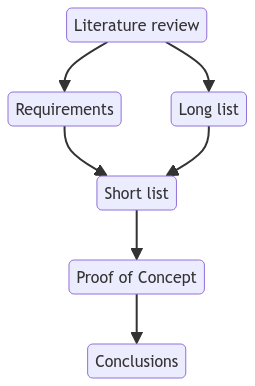
\includegraphics[height=.3\paperheight]{methodology.png}
    \caption{A flowchart representation of the methodology}
\end{figure}

The research will be divided into 6 phases, the first of which is a literature review. Literature research will be performed to examine existing approaches, explore popular languages, and gain a deeper understanding of the state of the art. The result of this literature search can be found in section 2 of this research proposal.

Phase 2 consists of creating a list of minimal requirements for a suitable language choice. Possible types of requirements could include ease of use, security implications, performance, and suitability for IAM-related tasks. A concrete list of measurable requirements will be assembled in consultation with thesis stakeholders and employees at TrustBuilder. The MoSCoW method will be used to order these requirements by importance, and each requirement will be marked as functional or non-functional.

Phase 3 is to create a long list of options, checked against the previously listed requirements. The literature review from phase 1 will be used to build an exhaustive list of suitable language choices. Popular existing options, as well as possibly lesser-known choices, will be considered.

Phase 4 aims to create a short list of the three most promising options, using a requirements summary table.

In phase 5, a proof of concept will be created to validate the suitability of each language in the short list. The proof of concept will consist of a simple HTTP server for each chosen language, which will allow running code that handles HTTP requests in the specified language. Three scripts will be written for each language, and will handle three distinct needs. The exact functionality of these three types of scripts will be decided based on TrustBuilder's typical customization requirements. This proof of concept will help further solidify and compare each language's suitability for customizing and extending IAM systems, and will provide deeper insight in their tooling and ease of use for these purposes.

Phase 6 will consist of drawing conclusions out of the research and propose next steps. The results and findings from the previous phases will be analyzed, and limitations and areas for future research will be identified.

Throughout this entire process, a thesis will be written that documents the research, findings, and proposed solutions.


%---------- Verwachte resultaten ----------------------------------------------
\section{Expected result, conclusion}%
\label{sec:expected_results}

Based on the findings in the literature review, JavaScript/TypeScript is expected to be the ideal language for writing extensions for IAM systems. It is currently the most popular programming language, and is already widely used for the extension of platforms, both in the general web development space as for IAM-related tasks. Being the most popular language, it has a rich package ecosystem, is actively being developed, and has a range of possible runtime environments. Having been specifically created for the web, with new standardized web APIs still being added, it can easily handle OAuth and SAML requirements, as both technologies were designed on top of existing web standards. JavaScript is already an excellent language choice for these purposes, and its continued innovation cements its place for years to come.

As many languages can be compiled to JavaScript or Wasm now, an extension system built on top of a JavaScript and Wasm engine would also enable the usage of other languages. A system that enables this level of versatility would provide a future-proof platform for mission-critical customization scripts.

